\documentclass{article}
\usepackage[utf8]{inputenc}
\usepackage{amsmath}
\usepackage{amssymb}
\usepackage{graphicx}
\usepackage{mathtools}


\graphicspath{{Images/}}

\setlength{\oddsidemargin}{0in}
\setlength{\textwidth}{6.5in}
\setlength{\topmargin}{-.55in}
\setlength{\textheight}{9in}
\pagestyle{empty}



\title{Scientific Computation HW4}
\author{Michael Nameika}
\date{October 2022}

\begin{document}

\maketitle

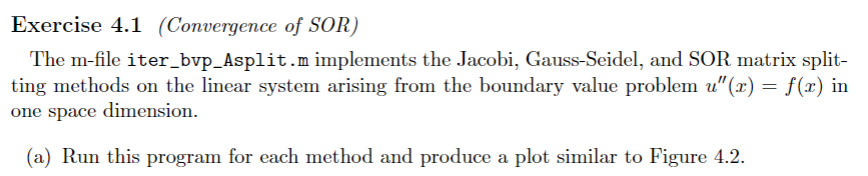
\includegraphics[scale = 0.8]{ex4.1a.PNG}
\newline
Running the iter\_bvp\_Asplit.m for the Jacobi, Gauss-Seidel, and Successive Overrelaxation methods, we find the following plot for each method's errors over the iterations:
\begin{center}
    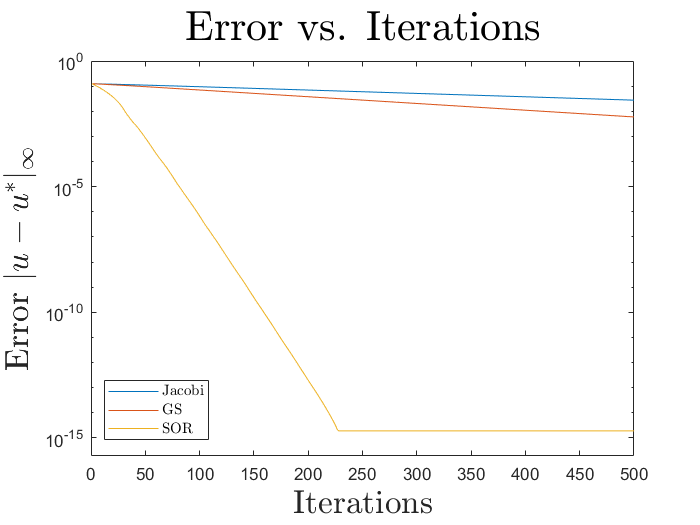
\includegraphics[scale = 0.6]{splittingErrors.png}
\end{center}

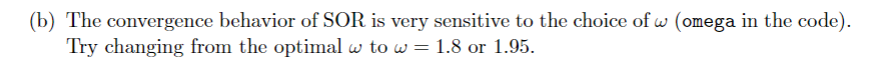
\includegraphics[scale = 0.8]{ex4.1b.PNG}
\newline

Changing the value of $\omega$ to 1.85 in the SOR method, we find the following plot of the error versus number of iterations:

\begin{center}
    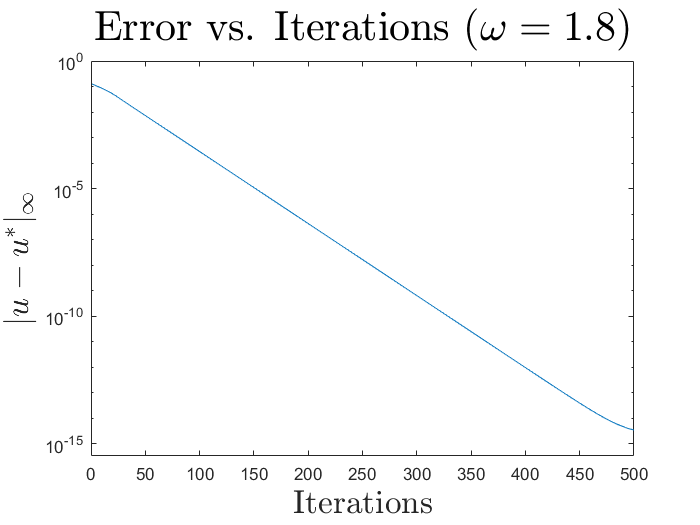
\includegraphics[scale = 0.6]{omega1.8.png}
\end{center}
And similarly for $\omega = 1.95$:

\begin{center}
    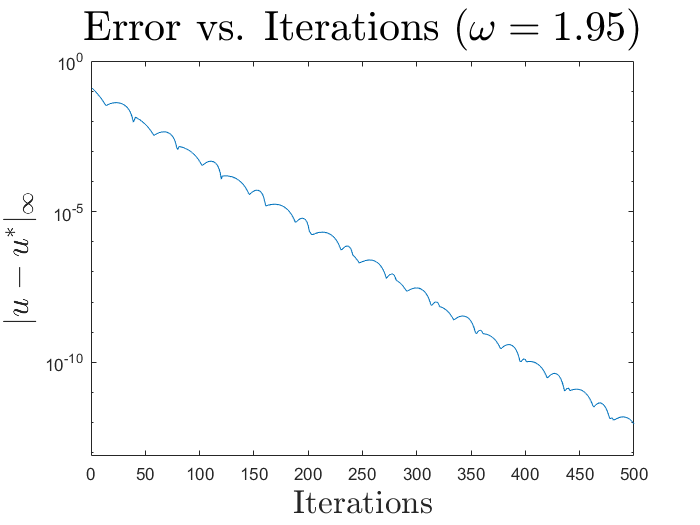
\includegraphics[scale = 0.6]{omega1.95.png}
\end{center}

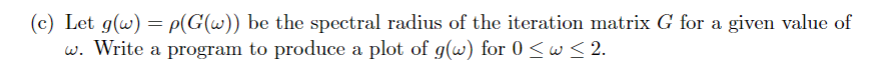
\includegraphics[scale = 0.8]{ex4.1c.PNG}
\newline

Using the modified code to run for values of $\omega$ between 0 and 2 using 101 mesh points, we find the following plot:

\begin{center}
    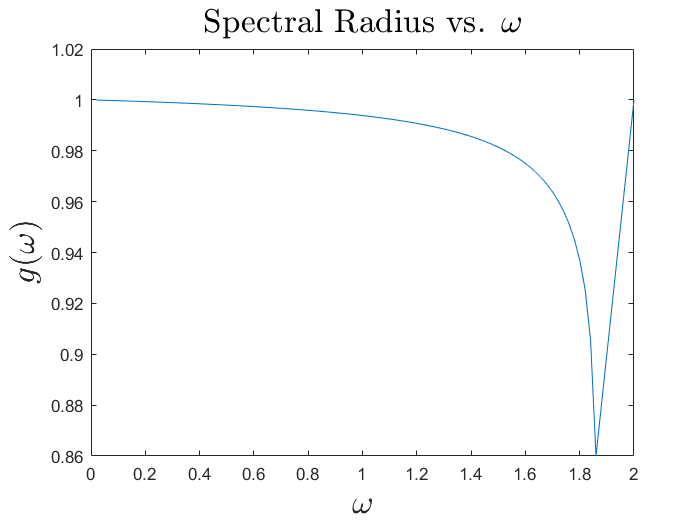
\includegraphics[scale = 0.6]{spectralRadiusvsOmega.png}
\end{center}


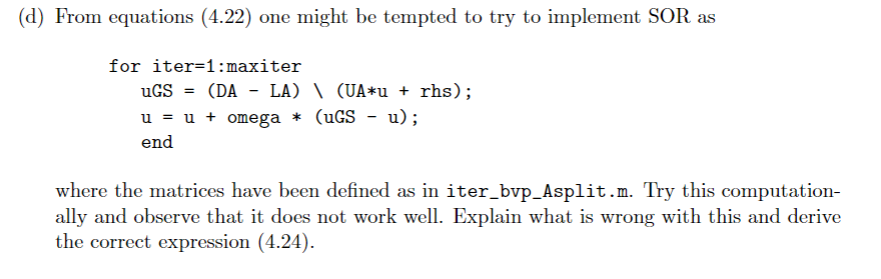
\includegraphics[scale = 0.8]{ex4.1d.PNG}
\newline

Implementing the above into the script, we find the following error plot and solution plot:

\begin{center}
    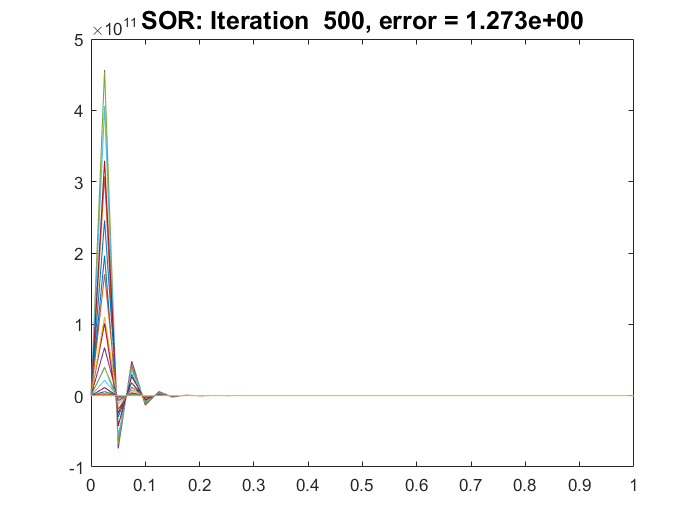
\includegraphics[scale = 0.4]{notworking.png}
    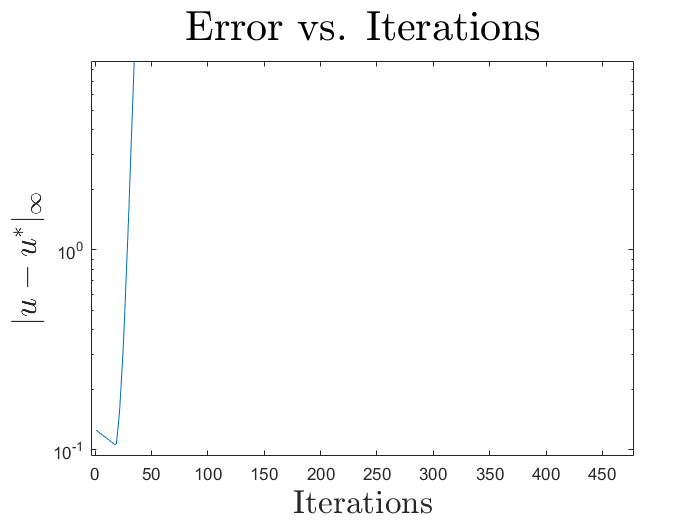
\includegraphics[scale = 0.4]{notworkingerror.png}
\end{center}

Clearly, this modification does not work. The reason this change does not work is because it does not account for the implicit steps. That is, we are assuming the Gauss-Seidel method is an explicit method for the SOR algorithm. This is clearly not the case, since Gauss-Seidel is implicit by definition! Let us derive the formula given by (4.24).
\newline
Recall the definition of the SOR method:
\[u_{ij}^{[k+1]} = u_{ij}^{[k]} + \omega(u_{ij}^{GS} - u_{ij}^{[k]})\]
where
\[u_{ij}^{GS} = \frac{1}{4}(u_{i-1,j}^{[k+1]} + u_{i+1,j}^{[k]} + u_{i,j-1}^{[k+1]} + u_{i,j+1}^{[k]}) - \frac{h^2}{4}f_{ij}\]
Substituting this into our definition for the SOR method, we find (after simplifying):
\[u_{ij}^{[k+1]} - \frac{\omega}{4}u_{i-1,j}^{[k+1]} - \frac{\omega}{4}u_{i,j-1}^{[k+1]} = (1 - \omega)u_{ij} + \frac{\omega}{4}u_{i+1,j}^{[k]} + \frac{\omega}{4}u_{i,j+1}^{[k]} - \frac{\omega h^2}{4}f_{ij}\]
Writing in matrix form, we find
\[-\frac{4}{\omega h^2}\begin{bmatrix}
    1 & & & & & \\
    -\omega /4 & 1 & & & \\
     & -\omega / 4 & 1 & & \\
     & & \ddots & \ddots & & \\
     & & & -\omega / 4 & 1\\
\end{bmatrix}U^{[k+1]} = -\frac{4}{\omega h^2}\begin{bmatrix}
    1-\omega & \omega /4 & & & & \\
     & 1-\omega & \omega /4 & & & \\
     & & \ddots & \ddots\\
     & & &1-\omega & \omega /4\\
     & & & & 1-\omega \\
\end{bmatrix} U^{[k]} + f_{ij}\]
which leads us to
\[M = \frac{1}{\omega}(D - \omega L) \:\: ; \:\: N = \frac{1}{\omega}((1-\omega)D + \omega U)\]
where
\[D = -\frac{4}{h^2}\begin{bmatrix}
    1 & & & & \\
     & 1 & & & \\
     & &\ddots & & \\
     & & & 1\\
\end{bmatrix} \:\: ; \: \: L = -\frac{4}{h^2} \begin{bmatrix}
    0 & & & & \\
    \omega / 4 & 0 & & & \\
    & \ddots & \ddots & & \\
    & & \omega / 4 & 0 \\
\end{bmatrix} \:\: ; \:\: U = -\frac{4}{h^2}\begin{bmatrix}
    0 & \omega /4 & & & \\
    & \ddots & \ddots & \\
    & & 0 & \omega /4 \\
    & & & 0 \\
\end{bmatrix}\]
Which is what we wished to show.
\newline\newline

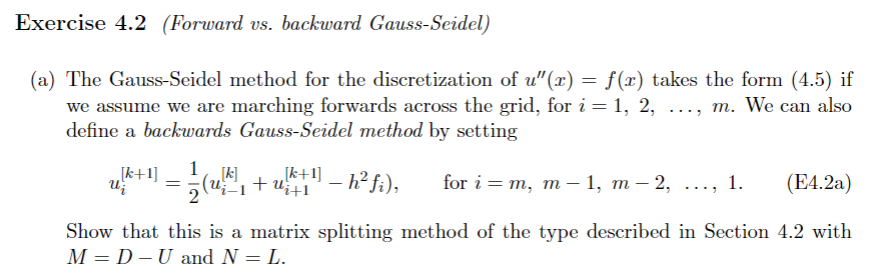
\includegraphics[scale = 0.8]{ex4.2a.PNG}
\newline

Rearranging the above equation, we find the following:
\[-\frac{2}{h^2}u_i^{[k+1]} + \frac{1}{h^2}u_{i+1}^{[k+1]} = f_i - \frac{1}{h^2}u_{i-1}^{[k]}\]
which we may write as
\[-\frac{1}{h^2}\begin{bmatrix*}[r]
    2 & -1 & & & \\
    & \ddots & \ddots & \\
    & & 2 & -1\\
    & & & 2 \\
\end{bmatrix*}U^{[k+1]} = -\frac{1}{h^2}\begin{bmatrix}
    0 & & & \\
    1 & 0 & &\\
    & \ddots & \ddots & \\
    & & 1 & 0\\
\end{bmatrix}U^{[k]} + f_i\]
Notice that this is a matrix splitting method for $M = D - U$ and $N = L$ where
\[D = -\frac{1}{h^2}\begin{bmatrix}
    2 & & & \\
    & 2 & & \\
    & & \ddots & \\
    & & & 2 \\
\end{bmatrix} \:\: ; \:\: U = -\frac{1}{h^2}\begin{bmatrix}
    0 & 1 & & \\
    & \ddots & \ddots & \\
    & & 0 & 1 \\
    & & & 0 \\
\end{bmatrix} \:\: ; \:\: L = -\frac{1}{h^2} \begin{bmatrix}
    0 & & & \\
    1 & 0 & & \\
     & \ddots & \ddots & \\
     & & 1 & 0 \\
\end{bmatrix}\]

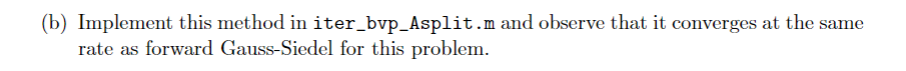
\includegraphics[scale = 0.8]{ex4.2b.PNG}
\newline

Swapping the position of $LA$ and $UA$ in the code (see code snippet below) 
\begin{center}
    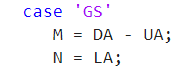
\includegraphics{forwardGS.PNG}
\end{center}
and running the forward Gauss-Seidel, we observe the following error plot for the forward and backward Gauss-Seidel methods:
\begin{center}
    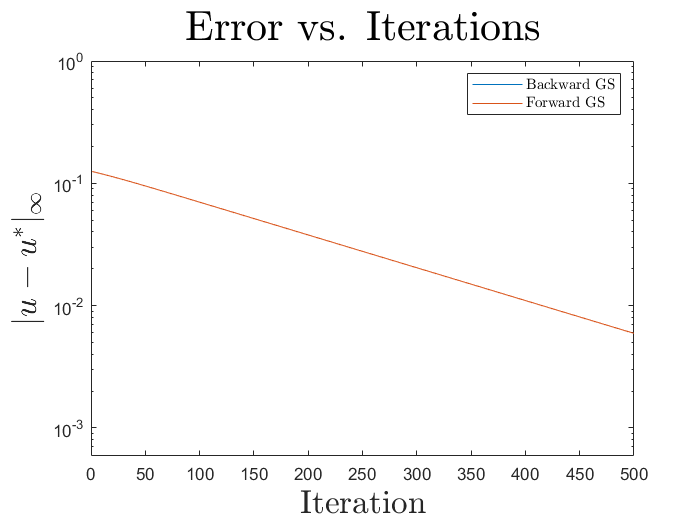
\includegraphics[scale = 0.6]{forward_backward_GS.png}
\end{center}
Notice that the error curve for the forward and backward Gauss-Seidel methods are indistinguishable.
\newline


\end{document}
